\chapter{Integración y despliegue continuo}
\label{chap:cicd}

\section{Objetivos del pipeline}
\label{sec:objetivos-pipeline}

El objetivo del pipeline es convertir el despliegue en un proceso repetible y auditable. Antes de desplegar, el sistema debe restaurar dependencias, compilar, ejecutar pruebas, construir la imagen Docker y validar Terraform. En el despliegue cloud, además, debe publicar la imagen en ECR, aplicar infraestructura, ejecutar migraciones y realizar pruebas de humo.

El pipeline se diseña para ejecución manual en \texttt{dev}. Esta decisión evita despliegues accidentales durante el desarrollo del TFG y permite capturar evidencias controladas.

\section{Validación automática}
\label{sec:validacion-automatica}

La validación automática incluye:

\begin{itemize}
  \item \texttt{dotnet restore} para restaurar dependencias.
  \item \texttt{dotnet build} para compilar la solución.
  \item \texttt{dotnet test} para ejecutar pruebas automatizadas.
  \item Validación de migraciones EF Core en el flujo de CI base.
  \item \texttt{docker compose config} para comprobar que la composición local es válida.
  \item \texttt{terraform fmt} y \texttt{terraform validate} para asegurar formato y coherencia de infraestructura.
  \item Validación de recursos de observabilidad tras el despliegue: log group, dashboard CloudWatch, alarmas y presencia de logs correlados.
\end{itemize}

\section{Publicación de artefactos}
\label{sec:publicacion-artefactos}

La imagen de la API se construye a partir de \path{TransitOps.Api/Dockerfile}. En el flujo de despliegue, la imagen se etiqueta con el identificador del commit o con un tag operativo, y se publica en el repositorio ECR \path{transitops/api}. En el despliegue real de Sprint 4 se publicó la imagen \path{sprint4-local-d00aa6b}. En la validación de Sprint 6 se publicó y desplegó la imagen \path{sprint6-local-6bb910c}.

ECR actúa como frontera entre construcción y ejecución: ECS no arranca una versión nueva de la API hasta que la task definition apunta a una imagen disponible.

\section{Despliegue automatizado}
\label{sec:despliegue-automatizado}

Se han definido dos workflows manuales:

\begin{itemize}
  \item \path{terraform-dev.yml}: inicializa Terraform, valida formato y configuración, genera plan y permite aplicar manualmente.
  \item \path{deploy-dev.yml}: ejecuta build, tests, construcción de imagen, publicación en ECR, Terraform, migraciones ECS, escalado del servicio, health check, bootstrap de administrador, login y verificaciones mínimas de observabilidad.
  \item \path{rollback-dev.yml}: reaplica Terraform con un tag de imagen conocido, espera estabilidad de ECS, comprueba que la task definition apunta a esa imagen y ejecuta un smoke test de readiness.
\end{itemize}

GitHub Actions accede a AWS mediante OIDC y asume un rol IAM de despliegue específico para TransitOps:

\begin{center}
{\small\path{transitops-dev-github-actions-deploy-role}}
\end{center}

No se utilizan claves AWS persistentes en GitHub. El rol mantiene permisos amplios para operar Terraform sobre \texttt{dev}, pero su trust policy limita la asunción al repositorio y rama configurados.

En Sprint 6 se amplió el workflow de despliegue para consumir variables de entorno relacionadas con observabilidad y DNS. La variable \texttt{ALARM\_EMAIL}, si existe en GitHub, se pasa a Terraform como \texttt{TF\_VAR\_alarm\_email} para crear una suscripción SNS de email. Cuando no se configura, Terraform crea las alarmas sin acciones de notificación, evitando depender de una dirección personal para que el entorno sea reproducible.

Después de aplicar infraestructura, el workflow captura outputs relevantes del módulo de observabilidad y comprueba que existen el grupo de logs, el dashboard y las alarmas esperadas. También busca logs JSON con un identificador de correlación generado durante el smoke test. Estas comprobaciones convierten la observabilidad en un criterio de despliegue, no en una revisión manual posterior.

En Sprint 7 se añadió un flujo de rollback explícito. La operación no reconstruye la aplicación ni cambia el contrato HTTP: recibe un \texttt{api\_image\_tag} ya publicado en ECR y lo convierte en el tag deseado de la task definition mediante Terraform. Esto deja el rollback trazable en el state, evita cambios manuales sobre ECS y permite comprobar que la imagen activa coincide con el tag esperado.

En Sprint 8 se cerró el camino de recreación completa del entorno \texttt{dev}. El procedimiento parte de un state vacío tras \texttt{terraform destroy}, aplica la plataforma con ECS a cero tareas, publica una imagen con tag operativo, carga secretos de runtime, ejecuta migraciones con \path{--migrate-only}, escala ECS a una tarea y valida HTTPS, login y observabilidad. La ejecución real usó el tag \tech{sprint8-good-fdf98b9} y una tarea de migración finalizada con exit code \texttt{0}. Este flujo convierte la reconstrucción del entorno en una operación documentada, no en una secuencia de pasos recordados de forma informal.

\begin{figure}[htbp]
\centering
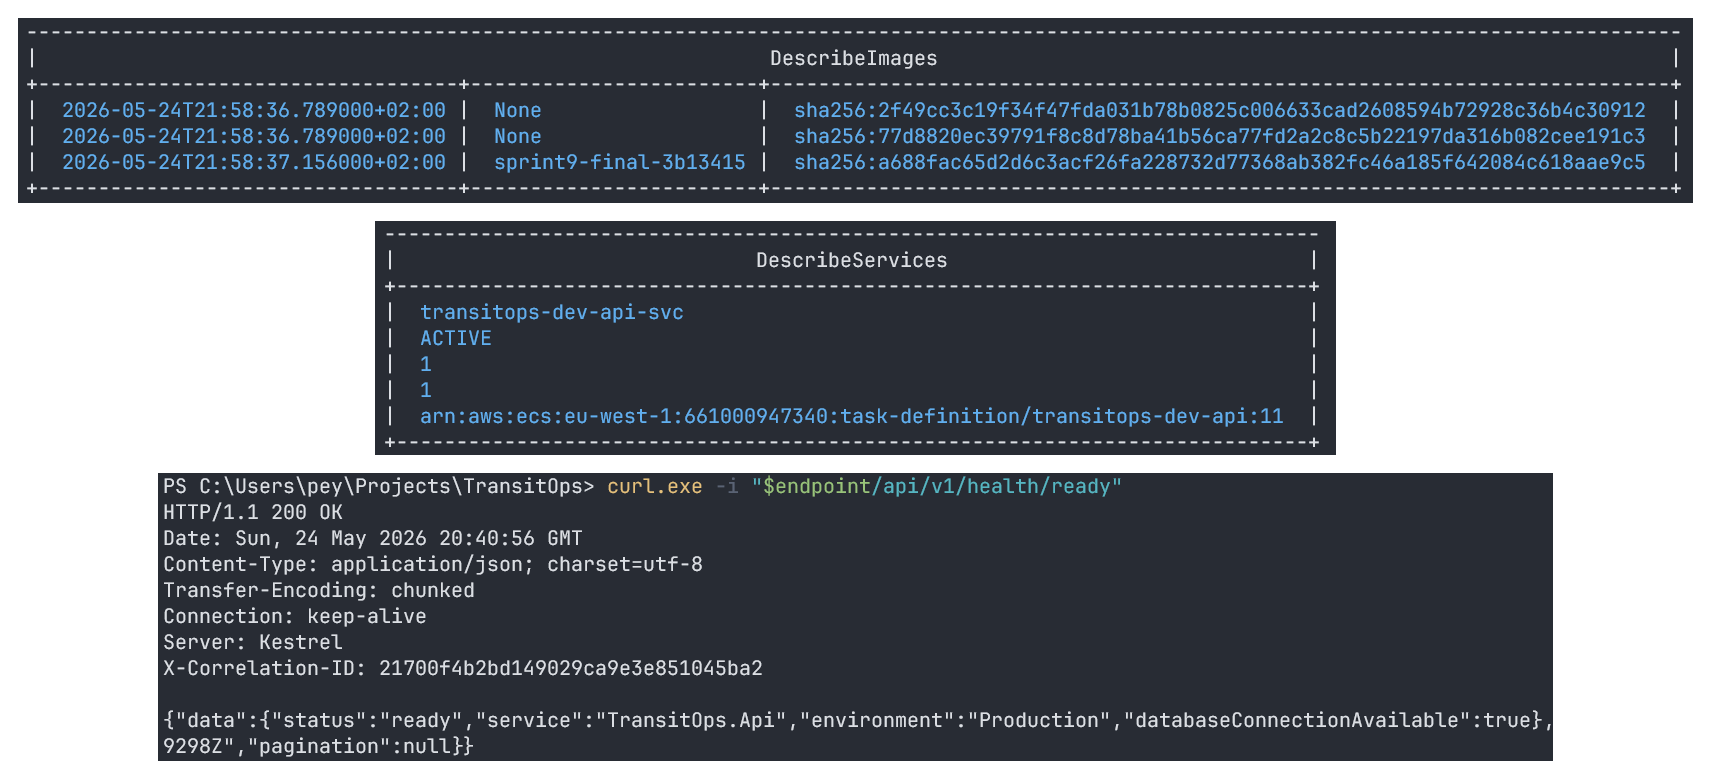
\includegraphics[width=0.92\textwidth]{imaxes/deploy-cloud-evidence}
\caption{Evidencia de despliegue cloud final: imagen publicada en ECR, servicio ECS estable y readiness HTTPS con respuesta 200.}
\label{fig:deploy-cloud-evidence}
\end{figure}

\begin{figure}[htbp]
\centering
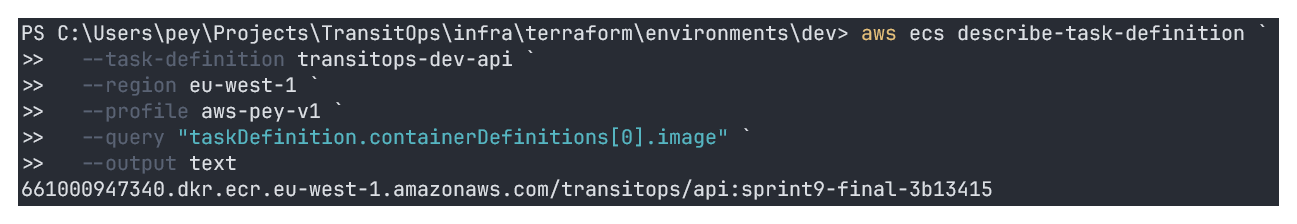
\includegraphics[width=0.92\textwidth]{imaxes/rollback-tag-evidence}
\caption{Verificación de la task definition activa apuntando al tag operativo validado.}
\label{fig:rollback-tag-evidence}
\end{figure}

\begin{figure}[htbp]
\centering
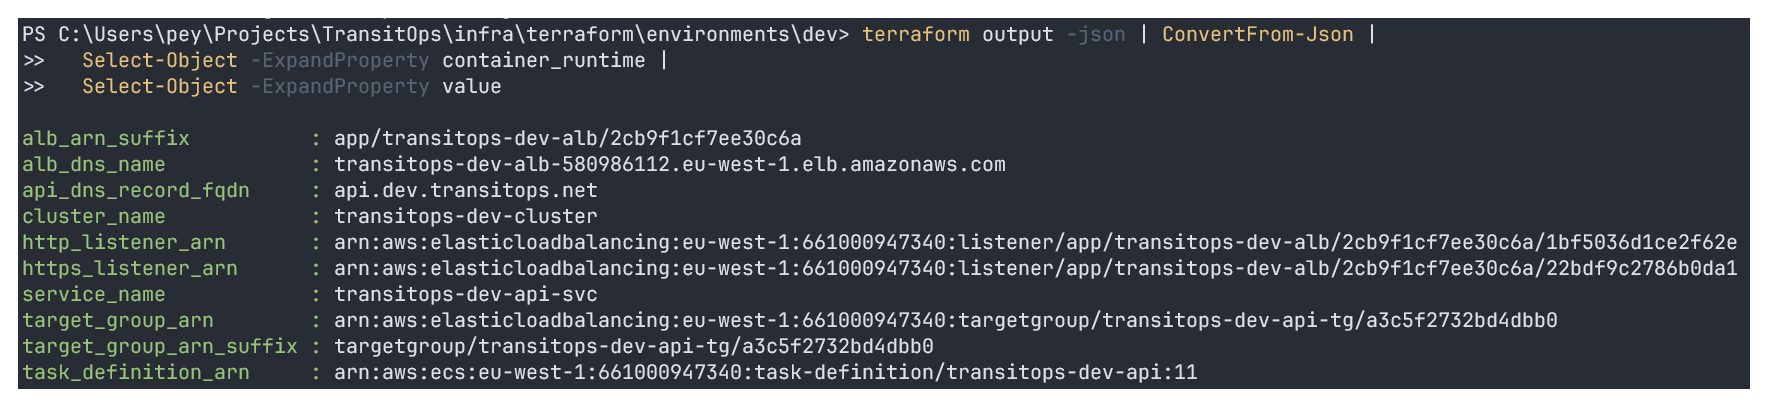
\includegraphics[width=0.92\textwidth]{imaxes/recreate-terraform-outputs}
\caption{Outputs de Terraform tras la recreación del entorno dev, incluyendo ALB, DNS, ECS y task definition activa.}
\label{fig:sprint8-recreate}
\end{figure}
